\documentclass[10pt]{article}
\usepackage{graphicx}
\usepackage[utf8]{inputenc}
\usepackage[T1]{fontenc}
\usepackage[brazilian]{babel}
\usepackage{comment} 
\usepackage{geometry}
\geometry{
    a4paper,
    total={170mm,257mm},
    left=20mm,
    top=20mm,
 }
\setlength{\parindent}{4em}
\setlength{\parskip}{1em}
\renewcommand{\baselinestretch}{1.2}

\title{Listão P2 Redes}
\author{Guilherme Christopher Michaelsen Cardoso}

\begin{document}

\maketitle

\begin{enumerate}
    \item \textbf{Conceitue a gerência de redes OSI com detalhes (mostrando desenhos)
    com os principais componentes e da arquitetura de gerência OSI. Quais
    são as principais características da gerência de redes SNMP (considere
    também os conhecimentos adquiridos na realização do segundo trabalho
    prático)? }
        \par
        Gerência de Redes é uma aplicação distribuída, onde 
        processos de gerência (agente-gerente) trocam informações entre si
        com o objetivo de monitorar e controlar a rede. O 
        Processo Gerente envia solicitações ao 
        rocesso Agente, que por sua vez responde as solicitações
        e envia notificações ao processo gerente. Para responder as solicitações
        o Processo Agente consulta uma MIB, ou seja, uma Base de
        Informações Administrativas, onde ficam armazenadas as informações
        da rede que são estruturadas em forma de árvore, seguindo o 
       paradigma de orientação a objetos, onde objetos gerenciados
        representam os recursos da rede.

        O SNMP (Simple Network Management Protocol) é um protocolo padrão
        da Internet para gerenciamento de dispositivos em redes IP. Ele é
        usado em sistemas de gerenciamento de rede para monitorar dispositivos
        ligados a rede para condições que garantem atenção administrativa.
        O SNMP é um componente do conjunto de protocolos da Internet como
        definido pela IETF. Ele consiste de um conjunto de padrões de 
        gerenciamento de rede, incluindo um protocolo da camada de aplicação,
        um esquema de banco de dados, e um conjunto de objetos de dados.
        
        O software de gerência de redes \textbf{não} segue o modelo
        cliente-servidor convencional. Por conta disso, os sistemas de gerência
        de redes evitam os termos 'cliente' e 'servidor' e optam por usar
        "gerente" para a aplicação que roda na estação de gerenciamento
        e "agente" para a aplicação que roda no dispositivo de rede.

        Uma rede gerida pelo protocolo SNMP é formada por três componentes
        chaves:
        
        \begin{itemize}
            \item Dispositivos Geridos
            \item Agentes
            \item Sistema de Gerenciamento de Redes (NMS - Network
                Management Systems)
        \end{itemize}
       
        Um Dispositivo Gerido é um nó de rede que possui um agente SNMP 
        instalado e se encontra numa rede gerida. Estes dispositivos coletam
        e armazenam informações de gestão e mantém essas informações disponíveis
        para sistemas NMS através do protocolo SNMP. Dispositivos geridos, também
        às vezes denominados de dispositivos de rede, podem ser routers, servidores
        de acesso, impressoras, computadores, servidores de rede, switches, 
        dispositivos de armazenamento, dentre outros.

        Um Agente é um módulo de software de gestão de rede que fica armazenado
        num Dispositivo Gerido. Um Agente tem o conhecimento das informações
        de gestão locais e traduz estas informações para um formato compatível
        com o protocolo SNMP.

        Um sistema NMS é responsável pelas aplicações que monitoram e controlam
        os dispositivos Geridos. Normalmente é instalado num (ou mais que um)  servidor de rede dedicado a estas operações de gestão, que recebe 
        informações (pacotes SNMP) de todos os dispositivos geridos daquela
        rede. 
        
    \begin{figure}[h!]
        \centering
         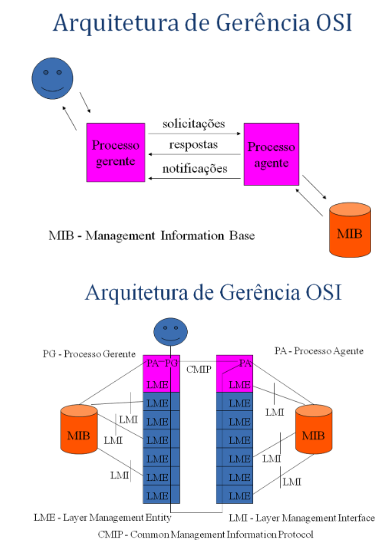
\includegraphics[width=80mm]{figura.png}
        \label{fig:figura1}
    \end{figure}
    
    \item \textbf{Comente sobre as cinco áreas funcionais da gerência de redes e
    serviços (Gerência de Configuração, Falhas, Desempenho, Segurança e
    Contabilidade), considerando ai mplantação e uso de uma rede de computadores
    em conformidade com o plano de negócios(atividades) da empresa(instituição).}

    \textit{
        \begin{itemize}
            \item \textbf{Gerência de Configuração:} Após a fase de
                planejamento, ocorrerá a aquisição de recursos para
                "configuração" dos dispositivos de hardware e software,
                estabelecendo políticas e mecanismos para fazer atualizações
                e auxiliar no correto funcionamento da rede de computadores.
            \item \textbf{Gerência de Falhas:} Tem como objetivo principal
                estabelecer mecanismos e políticas para detectar e reparar
                falhas, atuando em cooperação com a gerência de configuração
                e desempenho.
            \item \textbf{Gerência de Desempenho:} Medir o desempenho dos
                recursos e serviços da rede de computadores, estabelecendo
                políticas e mecanismos para fazer a rede funcionar com certa
                garantia (confiabilidade). A gerência de desempenho pode 
                contribuir pró-ativamente para manter a rede sempre funcionando,
                inclusive resolvendo os problemas de falhas. Isso ocorrerá
                com o auxílio de ferramentas de inteligência artificial.
            \item \textbf{Gerência de Segurança:} Estabelecer políticas e 
            mecanismo para tratar dos aspectos de segurança da sua estrutura
            de redes de computadores, em conformidade com os objetivos das 
            instituições.
            \item \textbf{Gerência de Contabilidade:} Estabelecer politicas
            e mecanismos para valorar(quantificar) e medir o uso dos recursos
            e serviços de redes de computadores e telecomuniações.
        \end{itemize}
    }

    \item Comente sobre as sete unidades de dados do protocolo ou operações de
    gerência de redes do SNMP (Simple Network Management Protocol): GetRequest,
    SetRequest, GetNextRequest, GetBulkRequest, Response, Trap e InformRequest
    
    \begin{itemize}
        \item \textbf{GetRequest:} Uma requisição de gerente a agente para
        obter o valor de uma variável ou lista de variáveis. As variáveis
            desejadas são especificadas em bindings de variaveis (valores
            não são usados). A obtenção dos valores das variáveis deve
            ser feita como uma operação atômica pelo agente. Uma
        \textit{Response} com os valores atuais é retornada.
        \item \textbf{SetRequest: } Uma requisição de gerente a agente para
        alterar o nome de uma variável ou lista de variáveis. Os bindings
        de variáveis são especificados no corpo da requisição. Mudanças
        a todas as variáveis especificadas devem ser feitas como uma
        operação atômica pelo agente. Uma \textit{Response} com os
        novos valores atuais das variáveis é retornada.
        \item \textbf{GetNextRequest: } Uma requisição de gerente a agente
        para descobrir variáveis disponíveis e seus valores. Retorna uma
        \textit{Response} com o binding da variável para a variável 
        lexicograficamente mais próxima disponível no MIB. O MIB
        inteiro de um agente pode ser percorrido pela aplicação iterativa
        de \textit{GetNextRequest}, começando à partir do OID 0. Linhas de uma tabela podem ser lidas especificando OIDs de colunas nos
        bindings de variáveis da requisição. Os campos PDU específicos 
        \textit{non-repeaters} and \textit{max-repetitions} são usados para controlar
        o comportamento da resposta. \textit{GetBulkRequest} foi introduzido no
        SNMPv2.
        \item \textbf{GetBulkRequest: } Versão otimizada do \textit{GetNextRequest}.
        Uma requisição de gerente a agente para múltiplas iterações do \textit{
        GetNextRequest}. Retorna uma \textit{Response} com múltiplos bindings de
        variáveis percorridas através dos bindings da requisição. Os campos PDU
        específicos \textit{non-repeaters} e \textit{max-repetitions} são usados
        para controlar o comportamento da resposta. \textit{GetBulkRequest} foi
        introduzido no SNMPv2.
        \item \textbf{Response: } Retorna bindings de variáveis e reconhecimento
        do agente ao gerente para \textit{GetRequest, SetRequest, GetNextRequest,
        GetBulkRequest e InformRequest.} Reporting de erros é provido pelos campos
        \textit{error-status} e \textit{error-index}. Apesar de ser usado como
        resposta tanto nos gets e sets, este PDU era chamado \textit{GetResponse} no
        SNMPv1.
        \item \textbf{Trap} Notificação assíncrona de agente a gerente. Traps SNMP
        habilitam um agente a notificar a estação de gerenciamento de eventos 
        significativos na forma de uma mensagem SNMP não solicitada. Inclui o 
        valor atual de \textit{sysUpTime}, um OID identificando o tipo de trap
        e bindings de variáveis opcionais. O endereçamento de destino dos traps
        é determinado de uma forma específica da aplicação, tipicamente através
        de configuração de variáveis trap no MIB. Enquanto na comunicação clássica
        o cliente requisita ativamente informação do servidor, o SNMP permite o uso 
        das traps. Esses são pacotes de dados enviados do servidor SNMP para o cliente
        sem que sejam explicitamente requisitados.
        \item \textbf{InformRequest}: Notificação síncrona reconhecida. Este PDU
        foi introduzido em SNMPv2 e foi originalmente definido como uma comunicação
        de gerente a gerente. Implementações posteriores permitem comunicações
        de agente a gerente. Notificações de gerente a geretne já eram possíveis em
        SNMPv1 (usando um \textit{Trap}), mas como o SNMP normalmente roda via
        UDP onde a entrega não é assegurada e pacotes perdidos não são reportados,
        a entrega de um Trap não era garantida. \textit{InformRequest} conserta 
        isso enviando uma confirmação no recebimento.
    \end{itemize}

    \item Comente sobre os primeiros RFCs (Request for Comments) para o SNMP, 
    também conhecido como SNMPv1, que apareceram em 1988: (RFC 1065- Structure
    and identification of management information for TCP/IP-based internets;
    RFC 1066 - Management information base for network management of TCP/IP
    based internets; RFC 1067 - A simple network management protocol)

    \begin{enumerate}
        \item RFC 1065 - Este RFC provê as definições comuns para a estrutura e
        identificação de gerenciamento de informação para internets baseadas
        em TCP/IP. Ele provê uma arquitetura simples e um sistema para gerenciar
        as redes TCP/IP, em particular a Internet. 

        \item RFC 1066 - Este RFC trata da versão inicial da base de dados
        de gerenciamento de informação (MIB) para uso conjunto com protocolos
        de gerência de redes em internets baseadas em TCP/IP.

        \item RFC 1067 - Este RFC define um protocolo simples através do qual
        o gerenciamento de informação para um elemento de rede pode ser 
        inspecionado por usuários logicamente remotos. Ele provê uma 
        arquitetura simples para gerenciar internets baseadas em TCP/IP, em especial,a
        Internet.
    \end{enumerate}

    \item Apresente os elementos de serviços da camada de aplicação OSI envolvidos 
    com as operações de gerência de redes e as respectivas primitivas relacionadas
    com a operação de gerência GET

    \item Comente sobre os três principais modelos de serviços e os quatro modelos
    de implantação relacionados com computação em nuvem (cloud computing).
    \textbf{Modelos de serviços: }
    \begin{itemize}
        \item \textbf{SaaS - Software as a Service}:
        É um modelo onde a aquisição e/ou utilização de um software não está 
        relacionado a compra de licenças, ou seja, você utiliza algum software e 
        paga por sua utilização. 
        \item \textbf{IaaS - Infrastructure as a Service}:
        De forma análoga ao SaaS, neste modelo você contrata sua infraestrutura
        como serviço, por exemplo, ao invés de adquirir hardware, servidores,
        roteadores, etc, você contrata servidores virtuais e outros dispositivos
        de infraestrutura.
        \item \textbf{PaaS - Platform as a Service}:
        Aqui temos um modelo que fica entre o SaaS e IaaS, proporcionando uma
        plataforma mais robusta e flexível para a utilização de muitos recursos
        de tecnologia, onde é possível a utilização de software sde maneira mais 
        flexível, sendo possível desenvolver suas próprias aplicações baseadas
        em alguma tecnologia e utilizar a infraestrutura necessária, e o mais
        importante, adequada a aplicação desenvolvida.
    \end{itemize}
    \textbf{Modelos de Implantação:}
    \begin{itemize}
        \item \textbf{Nuvem Privada:} As nuvens privadas são aquelas construídas
        exclusivamente para um único usuário (uma empresa, por exemplo). 
        Diferentemente de um data center privado virtual, a infraestrutura utilizada
        pertence ao usuário, e portanto ele possui total controle sobre como as 
        aplicações são implementadas na nuvem. Uma nuvem privada é, em geral,
        construída sobre um data center privado.
        \item \textbf{Nuvem pública:} Uma nuvem é chamada de "núvem pública" quando
        os serviços são apresentados por emio de uma rede que é aberta para uso 
        público. Serviços de nuvem pública podem ser livres. Tecnicamente pode
        haver pouca ou nenhuma diferença entre a arquitetura de nuvem privada e
        públicak, entretanto, considerações de segurança podem ser substancialmente
        diferentes para os serviços (aplicações, armazenamento e outros recursos) que
        são disponibilizados por um provedor de serviços para um público e quando 
        a comunicação é afetada sobre uma rede não confiável. Geralmente, provedores
        de serviços de nuvem pública como a Amazon AWS, Microsoft e Google possuem
        e operam a infraestrutura em seus centros de dados e o acesso geralmente
        é feito por meio da Internet. A AWS e a Microsoft também oferecem serviços
        contectados diretamente chamados "AWS Direct Connect" e "Azure ExpressRoute"
        respectivamente. Tais conexões necessitam que os clientes comprem ou aluguem 
        uma conexão privada a um ponto de troca de tráfego oferecido pelo provedor
        de nuvem. 
        As aplicações de diversos usuários ficam misturadas nos sistemas de 
        armazenamento, o que pode parecer ineficiente a princípio. Porém, se 
        a implementação de uma nuvem pública considera questões fundamentais, como
        desempenho e segurança, a existência de outras aplicações sendo executadas
        na mesma nuvem permanece transparente tanto para os prestadores de serviços
        quanto para os usuários.
        \item \textbf{Nuvem comunitária}: A infraestrutura de nuvem é compartilhada
        por diversas organizações e suporta uma comundiade específica que partilha
        as preocupações (por exemplo, a missão, os requisitos de segurança, política
        e considerações sobre o cumprimento). POde ser administrado por organizações
        ou por um terceiro ep ode existir localmente ou remotamente.
        \item \textbf{Nuvem híbrida}: Nas nuvens híbridas temos uma composição dos
        modelos de nuvens públicas e privadas. Elas permitem que uma nuvem privada
        possa ter seus recursos ampliados a partir de uma reserva de recursos em 
        uma nuvem pública. Essa característica possui a vantagem de manter os níveis
        de serviço mesmo que haja flutuações rápidas na necessidade dos recursos. 
        A contexão entre as nuvens pública e privada pode ser usada até mesmo em
        tarefas periódicas que são mais facilmente implementadas nas nvuens públicas,
        por exemplo. O termo computação em ondas é, em geral, utilizado quando se
        refere às nuvens híbridas.
    \end{itemize}

    \item Comente sobre as funções das três principais camadas (view, integration
    and infrastructure layers) da arquitetura PCMONS (Private Cloud Monitoring
    System).



    \item Descreva sucintamente as atividades relacionadas ao projeto e desenvolvimento
    de protocolos (especificação informal, especificação formal, validação, 
    verificação, implementação e teeste) descrevendo as relações existentes entre estas
    atividades. Para explicitar melhor, apresente também um desenho destas atividades e
    relações 

    \begin{enumerate}
        \item \textbf{Especificação informal:} Especificação inicial do protocolo,

    \end{enumerate}

    \item Observe a especificação através de modelos de transição [MEF (Maquina 
    de Estados Finitos)] realizada abaixo para o protocolo de enlace de dados entre
    as duas interfaces de uma rede local, onde o controle de fluxo empregado é do tipo
    envia-espera e após enviar um quadro de dados a emissora aguarda a chegada do seu
    reconhecimetno.
    \begin{enumerate}
        \item Considerando a transmissão de um QU (Quadro de Usuário) da máquina 1 
        para máquina 2 descreva o que acontece em cada transição realizada pelas MEF,
        citando os elementos dos conjuntos de entrada e saída envolvidos, desde
        o recebimento de QU no BE1 da máquina 1 até o recebimento do ACKIN no BE2 da
        máquina 1.
        \item Considerando a chegada de DADOIN na máquina 2, mostre como é acionada
        a "temporização" na máquina 1 e reenviado o DADOOUT, apresentando as transições
        com seus respectivos elementos dos conjuntos de entrada e saída da MEF 
        envolvidos; também explique sobre o que acontece na ocorrência de cada 
        transição. 
        \item Comente sobre alguns problemas que podem ocorrer devido a simplicidade 
        deste protocolo (MEF), mostrando as transições com seus respecitvos elementos
        dos conjuntos de entrada e saída da MEF envolvidos para o exemplo de duplicação
        de dados recebidos.
        \begin{figure}[h!]
            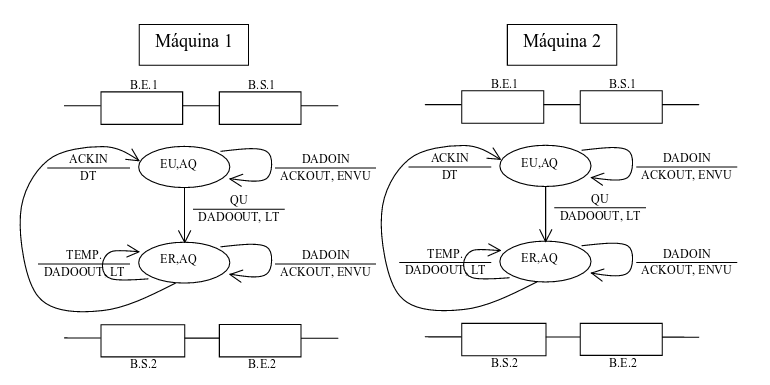
\includegraphics[width=\linewidth]{mef.png}
            \label{fig:mef1}
        \end{figure}
    \end{enumerate}
    \item O emprego de Modelos de Transição como técnica de especificação formal de
    protocolas apresenta alguns problemas. Para auxiliar nesta situação são utilizados
    também Linguagens de Programação e Modelos Mistos. Cite alguns problemas, 
    descrevendo em que sentidos as Linguagens de Programação e os Modelos Mistos podem
    auxiliar. Como as ferramentas de especificação formal, Lotos, Estelle, Z..., podem
    auxiliar para resolver os problemas os problemas mencionados acima?

    \item Concluída a verificação de especificação de um protocolo, chega o momento
    de implementá-lo nos vários sistemas da rede que irão utilizá-lo em suas 
    comunicações. A decisão de como integrar a implementação de um protocolo no 
    sistema local se assenta nos seguintes objetivos, relativos ao nível de desempenho
    desejado: minimizar custo do serviço de comunicação; maximizar vazão nas conexões
    utilizadas; minimizar a utilização dos recursos do sistema dedicados à comunicação.
    Tendo em vista esses objetivos, a implementação pode ser integrada de três 
    maneiras. Quais são estas maneiras? Comente um pouco sobre cada uma destas
    maneiras.

    \item Quais são as principais topologias de redes locais existentes? Apresente
    desenhos e comentários sobre as topologias relacionadas aos padrões IEEE 802.3,
    802.4 e 802.5.

    \item Comente sobre os protocolos IEEE 802.3 - CSMA/CD (Carrier Sense Multiple
    Access with Collision Detection) para barramento (apresente um fluxograma),
    IEEE 802.4 - "token bus" e IEEE 802.5 - "token ring".

    \item \textbf{O que é chaveamento de pacotes e de circuitos? Comente sobre as 
    vantagens de cada tipo de chaveamento.}
    \begin{itemize}
        \item Chaveamento de pacotes: Mensagem dividida em pequenos pacotes
        que são enviados da origem ao destino, apssando por roteadores intermediários.
        Os caminhos a serem percorridos dependem do "controle de congestionamento".
        \item Chaveamento de circuitos: Nesse caso teremos um único caminho a ser
        percorrido por todos os pacotes. Para isso, devemos alocar "circuitos" entre
        osroteadores, ou "comutadores", escolhendo o "circuito" mais adequado em
        conformidade com os parâmetros de qualidade de serviço desejados.
    \end{itemize}

    \textbf{Vantagens: } NO CP temos que considerar o melhor esforço (best effort),
    que oferece baixo custo. No CC temos qualidade de serviço garantida, conforme
    desejado (solicitado).
    \textbf{Desvantagens: } No CP, com melhor esforço, a qualidade de serivço fica
    prejudicada a medida que o tráfego aumenta. No CC devemos "pagar" para ter
    a a garantia de seviços desejada.

    \item Ainda em relação a camada de rede comente sobre: roteamento, controle de 
    congestionamento, serviço não orientado e orientado a conexões. 

    \item Quantas redes estão disponíveis e quantos computadores podemos interconectar
    em cada classe de endereço (IPv4) da Internet?
    
    \textbf{Classe A}: \begin{math}2^7 - 2  = 126 \end{math} redes e 
    \begin{math}2^{24} - 2 = 16777214 \end{math} dispositivos.
    
    \textbf{Classe B}: \begin{math}2^{14} = 16384 \end{math} redes e 
    \begin{math}2^{16} - 2 = 5534\end{math} dispositivos.
    
    \textbf{Classe C:} \begin{math}2^{21} = 2097152 \end{math} redes e 
    \begin{math}2^8 - 2  = 254 \end{math}
\end{enumerate}
\end{document}
